%\documentclass{article}
\documentclass[a4paper,12pt]{article}
% Seitenränder in schön für Steven
\usepackage[paper=a4paper,left=25mm,right=25mm,top=25mm,bottom=25mm]{geometry}
\usepackage{enumitem}
\usepackage{amsmath}
\usepackage{float}
\usepackage{graphicx}
\usepackage{tikz}
\usepackage{titling}
\usepackage{setspace}


% Schusterjungen und Hurenkinder bestrafen
\clubpenalty50000
\widowpenalty50000
\displaywidowpenalty=50000

% Buchstaben mit kringel drum: %
\newcommand*\mycirc[1]{%
	\begin{tikzpicture}[baseline=(C.base)]
	\node[draw,circle,inner sep=1pt](C) {#1};
	\end{tikzpicture}}

\newcommand*\red[1]{\textcolor{red}{#1}}

\author{Benedict Hans, Christoph Dollase, Steven Te\ss endorf}
\setlength{\droptitle}{-5em} % set the title to the top of the page

% ==========================
% ===== START HERE!! =======
% ==========================
\title{ \textbf{Problem Sheet 8}}
\setcounter{section}{8} % Nummer des Aufgabenblattes

\begin{document}	 
	\maketitle	 %Some Vodoo-magic
	
	\subsection{Hamming Codes}
	\textbf{Assume you have to transmit messages of 256 bit length over a lossy channel, with a bit error probability of 0.1 \%, i.e.  every bit has a 1/1000 chance to flip}
	\begin{enumerate}[label=(\roman*),itemsep=0pt]
		\item \textbf{What is the propability for a correct transmission of 256 bits (without any error correction mechanism)?}
		\begin{itemize}[itemsep=0pt]
			\item $1 - (256 \cdot 0.1\%) = 1 - 0,256 = 0,744 \rightarrow  74,4\%$
			
		\end{itemize}
		\item \textbf{Assume you apply a Hamming Code to correct transmission errors. How many parity bits do you append to the message?  What is the resulting message length?}
		\begin{itemize}[itemsep=0pt]
			\item n = 256 (data bits) : $n = 2^k - k - 1$ , with k=8 only 247, add parity bit
			\item k = 9 (parity bits)
			\item N = 265 (message bits)
		\end{itemize}
		\item \textbf{What is the propability of a correct transmission now?}
		\begin{itemize}[itemsep=0pt]
			\item \red{$p_{korr} = p_{0Bit} + p_{1Bit} $}
			\item \red{$p_{korr} = (1-p)^{265} + (1-p)^{n-1} \cdot n \cdot p = 0,97$}
			\item Do we have to concider 2- and more-bit errors ?
		\end{itemize}
	\end{enumerate}

	
	\subsection{Hamming-Code}
	\textbf{Two entities have agreed to use the following encoding to transmit characters}
	\begin{enumerate}[itemsep=0pt]
		\item \textbf{How many check bits are required to correct all 1-bit errors in messages with a length of m bits?}
		\begin{itemize}[itemsep=0pt]
			\item $m = 2^k - k - 1 $
			\item $m + 1 = 2^k - k $
			\item $k = truncate(\log_2(m+\log_2(m))) + 1$
			\item e.g. you have 1337 bits of data:\\
			\textcolor{blue}{ $k = trunc(\log_2(1337 + \log_2(1337))) + 1$\\
			$k = trunc(\log_2(1337 + 10,3848)) + 1 = trunc(\log_2(1347,3848)) + 1$\\
			$k = trunc(10,3959) + 1 = 10 + 1 = \textbf{11}$}
		\end{itemize}
		\item \textbf{A Hamming Code with 4 check bits shall be used in the following.  Create the code words which represent the word HAMMING.}
		\begin{itemize}[itemsep=0pt]	
			\item Parity bit 0 (1): is XOR from Data bits 0, 1, 3, 4, 6 (3,5,7,9,11 $\rightarrow$ see slides) 
			\item Parity bit 1 (2): is XOR from Data bits 0, 2, 3, 5, 6 (3,6,7,10,11) 
			\item Parity bit 2 (4): is XOR from Data bits 1, 2, 3 (5,6,7)
			\item Parity bit 3 (8): is XOR from Data bits 4, 5, 6 (9,10,11)
		\end{itemize}
		\begin{tabular}{c|c|ccccccccccc}
			~ & ~ & 1 & 2 & 3 & 4 & 5 & 6 & 7 & 8 & 9 & 10 & 11 \\
			Letter & binary & $p_0$ & $p_1$ & $d_0$ & $p_2$ & $d_1$ & $d_2$ & $d_3$ & $p_3$ & $d_4$ & $d_5$ & $d_6$ \\ \hline
			H & \textcolor{blue}{$[1001000]$} & \textcolor{red}{0} & \textcolor{red}{0} & 1 & \textcolor{red}{1} & 0 & 0 & 1 & \textcolor{red}{0} & 0 & 0 & 0 \\
			A & \textcolor{blue}{$[1000001]$} & \textcolor{red}{0} & \textcolor{red}{1} & 1 & \textcolor{red}{0} & 0 & 0 & 0 & \textcolor{red}{1} & 0 & 0 & 1 \\
			M & \textcolor{blue}{$[1001101]$} & \textcolor{red}{0} & \textcolor{red}{1} & 1 & \textcolor{red}{1} & 0 & 0 & 1 & \textcolor{red}{0} & 1 & 0 & 1 \\
			M & \textcolor{blue}{$[1001101]$} & \textcolor{red}{0} & \textcolor{red}{1} & 1 & \textcolor{red}{1} & 0 & 0 & 1 & \textcolor{red}{0} & 1 & 0 & 1 \\
			I & \textcolor{blue}{$[1001001]$} & \textcolor{red}{1} & \textcolor{red}{1} & 1 & \textcolor{red}{1} & 0 & 0 & 1 & \textcolor{red}{1} & 0 & 0 & 1 \\
			N & \textcolor{blue}{$[1001110]$} & \textcolor{red}{1} & \textcolor{red}{0} & 1 & \textcolor{red}{1} & 0 & 0 & 1 & \textcolor{red}{0} & 1 & 1 & 0 \\
			G & \textcolor{blue}{$[1000111]$}  & \textcolor{red}{1} & \textcolor{red}{1} & 1 & \textcolor{red}{0} & 0 & 0 & 0 & \textcolor{red}{1} & 1 & 1 & 1 \\
		\end{tabular}
	\\
		\item \textbf{Consider the following code words have been received:	\\
		\textcolor{blue}{$[010101000~ 111001000~ 010101001~ 001011000~ 111111100~ 001001100]$} 
		Decode  this  sequence,  mark  the  blocks  that  contain  an  error,  and  correct  the  errors  if possible.}
		\begin{itemize}[itemsep=0pt]
			\item \textcolor{blue}{$[010101000~ 11100\red{\mycirc{0}}000~ 01010100\red{\mycirc{0}}~ 001011000~ 111111100~ 0\red{\mycirc{1}}1001100]$}
			\item \red{D, \mycirc{A}, \mycirc{D} ,G ,O ,\mycirc{M} $\rightarrow$ \mycirc{$\Psi$} means, an error was correted}
		\end{itemize}
	\end{enumerate}
	
	
	% Solution
	
	\subsection{Efficiency of Stop-and-Wait}
	\textbf{Assume a channel with a bit rate of 1 Mbps and a delay of 20 ms.  A Stop-and-Wait protocol is used which unfortunately introduces waiting times and thus a low efficiency.  The efficiency is dependent on the size of the frames.  Determine the frame size for which the efficiency is 50\%.}\\
	
	\begin{itemize}[itemsep=0pt]
		\item with the use of the Stop-and-Wait protocol there os only one frame on the line at a time
		\item an acknowledgement has to arrive before the next frame is sent
		\item we need to assume that
		\begin{itemize}[itemsep=0pt]
			\item processing times are negligible 
			\item acknowledgements are always piggybacked
			\item packets in both directions have the same size
		\end{itemize}
	\end{itemize}
	
	\begin{minipage}{0.49\linewidth}
		\begin{doublespace}
			$efficiency = \frac{length}{(length + bitrate \cdot RTT)} $ \\ RTT = round trip time\\
			$\rightarrow 0.5 = \frac{length}{(length + 10^6 [bps]  \cdot  40 \cdot 10^{-3})} $ \\
			$\rightarrow 0.5 = \frac{length}{(length + 40 \cdot 10^3)}$ \\
			$\rightarrow length = 40~ kbits$
		\end{doublespace}
	\end{minipage}
	\hfill
	\begin{minipage}{0.49\linewidth}
			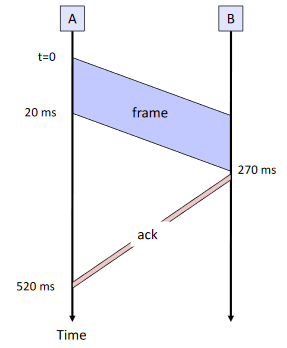
\includegraphics[width=0.5\linewidth]{Framesize.png}
	\end{minipage}
	

	% Solution 
	
	
	\subsection{Timers}
	\textbf{Explain the problem that is solved by timers. How can timers be implemented in software?}\\
	\\
	It is much easier to implement timeout functions etc.\\
	Some protocols require many timers, but only a couple hardware timers exist
	\begin{itemize}[itemsep=0pt]
		\item implement timers in software by using one hardware timer
		\item store expiration times in a linked list and update it during protocol time
		\item see slide 04.81 
	\end{itemize}
	\red{timers decides if the message should be send again, because we don't recognize if and where the message was lost}
	
	%Solution
	
	
\end{document}

% Hier nach passiert nichts mehr, daher nutzen wir das als kleines Cheat-Sheet ;)
% ===============================================================================

% Aufzählungen (auch merhstufig):
\begin{itemize}[itemsep=0pt]
	\item 
\end{itemize}

%Bilder eifnügen:
\begin{figure}[h!] %h! sorgt dafür dass das Bild möglichst nicht woanders hingeschoben wird
	%Erklärung: [width=0.5\linewidth] -> Bild ist maximal so breit wie die Hälfte des Schriftbildes
	\includegraphics[width=0.5\linewidth]{Bildname.jpg} 
	\caption{Bildunterschrift}
\end{figure}

%Tabelle einfügen:
\begin{table}[h!] %h! sorgt dafür dass die Tabelle möglichst nicht woanders hingeschoben wird
	\caption{Tabellenüberschrift}
	%hinter {tabular}: Anzahl Spalten (c=center, l=linksbündig, r=rechtsbündig, | Spaltenstriche)
	\begin{tabular}{|c|c|c} 
		A & B & C  \\ % \\ = return (neue zeile)
		\hline % horinzontale Linie
		0 & 1 & 2
	\end{tabular}
\end{table}
